% =====================================================================
% Section 2 -- Historical data and baseline audit
% Numbers in this section were extracted from the legacy Kaggle archives
% (Potato.zip, Potato_Improved.zip) by src/utils/legacy_audit.py.
% Tables are regenerated by src/utils/overleaf_sync.py.
% =====================================================================
\section{Dataset and Baseline Audit}
\label{sec:baseline_audit}

Before designing a new model we audited every artefact left by the earlier
experimental campaign: four Kaggle notebooks trained under a plain stratified
split (EfficientNet-B0, MobileViT-S, a sequential EfficientNet$\rightarrow$MobileViT
cascade and an EfficientNet$\rightarrow$Swin cascade) and a later, optimised
campaign that introduced a group-aware split, a policy screen, an architecture
screen and a final 5-fold cross-validation (CV). All metrics, per-epoch logs,
confusion matrices and duplicate reports were parsed directly from the archives;
model checkpoints were not needed for the analysis.

\subsection{Dataset composition and class imbalance}
\label{sec:audit_imbalance}

The Potato Leaf Disease Dataset in Uncontrolled Environment~\cite{shabrina2024dataset} contains
3{,}076 field photographs in seven classes (Table~\ref{tab:data_audit}).
The distribution is strongly skewed: \emph{Fungi} has 748 images while
\emph{Nematode} has only 68, an imbalance ratio of $11.0\times$; \emph{Healthy}
(201) is the second-smallest class. With five folds, each validation split
contains only 11--17 Nematode images, so a single misclassified sample moves
Nematode recall by 6--9 percentage points. This explains the large fold-to-fold
variance of minority-class metrics (Nematode F1 SD = 4.0\,pp for the selected
legacy model) and motivates reporting Macro-F1 alongside accuracy.

\input{tables/data_audit}

Class weighting was the single most effective intervention in the legacy policy
screen (Table~\ref{tab:legacy_policy}): square-root inverse-frequency weights
raised fold-1 Macro-F1 from 70.89\,\% to 74.65\,\% and Nematode recall from
34.4\,\% to 81.3\,\%. However, the final confusion matrices show the cost of this
re-weighting: pooled over five folds, Nematode recall reached 89.7\,\% but
precision only 67.0\,\%, because 14 Fungi and 9 Pest images were pushed into the
minority class. Healthy shows the same pattern (recall 86.1\,\%, precision
75.2\,\%), absorbing 27 Pest and 20 Virus images. The minority classes therefore
suffer from \emph{false positives}, not missed detections, which loss re-weighting
alone cannot fix.

\subsection{Byte-level and near-duplicate contamination}
\label{sec:audit_duplicates}

SHA-256 hashing found 110 files forming 55 groups of byte-identical images.
Six of these groups carry \emph{conflicting labels}: one Virus/Pest pair, one
Pest/Healthy pair, three Pest/Fungi pairs and one Pest/Nematode pair. Every
conflict involves the Pest class, which is also the class with the lowest
recall (75.6\,\%) and the dominant source of confusion with Fungi
(Section~\ref{sec:audit_confusion}). The same files are, in effect, annotated as
two diseases, so a perfect classifier cannot score 100\,\% on them, and if the
two copies are split across train and validation the model is penalised for
reproducing a training label.

The other 49 groups contain the same label twice. Thirty-eight of these
redundant copies belong to \emph{Phytophthora} and look like download artefacts
(\texttt{IMG\_9518.JPG} vs.\ \texttt{IMG\_9518 (1).JPG}). A 64-bit difference hash
(dHash) found a further 27 near-duplicate pairs with Hamming distance $\le 2$
(Fungi 9, Virus 7, Phytophthora 5, Bacteria 4, Pest 2), mostly consecutive burst
shots (\texttt{IMG\_1111} / \texttt{IMG\_1112}). None of them crosses classes.

The original four notebooks used \texttt{StratifiedKFold} on raw file paths, so
any duplicate or burst pair could appear in both the training and the validation
split. Their reported scores (Table~\ref{tab:legacy_cv}, ``Random'') are therefore
optimistically biased. Once the optimised campaign moved to a group-aware split,
MobileViT-S fell from $88.16\,\%$ to $83.68 \pm 1.42\,\%$ Macro-F1. That drop
should not be attributed to leakage alone: the two campaigns also differ in
learning rate (full fine-tuning at $10^{-3}$ vs.\ $2\!\times\!10^{-5}$ for the
backbone and $5\!\times\!10^{-4}$ for the head) and in training length (15 fixed
epochs vs.\ an early-stopped schedule capped at 14). We treat the group-aware
number as the only valid baseline.

\input{tables/legacy_cv}

\subsection{Confusion patterns}
\label{sec:audit_confusion}

Figure~\ref{fig:legacy_cm} shows the pooled 5-fold confusion matrix of the
selected legacy model (MobileViT-S, sqrt class weights, no augmentation). Errors
are concentrated in a small number of biologically plausible pairs:

\begin{itemize}
  \item \textbf{Pest $\leftrightarrow$ Fungi} is the largest error mode in both
  directions: 76 Pest images predicted as Fungi (12.4\,\% of Pest) and 69 Fungi
  images predicted as Pest (9.2\,\% of Fungi). Insect feeding damage and fungal
  necrosis both produce irregular brown lesions with chlorotic halos, and at
  $224\times224$ the fine cues that separate them (frass, feeding holes and leaf
  margins vs.\ concentric rings and sporulation texture) are only a few pixels
  wide. Three of the six label-conflicting duplicates are exactly Pest/Fungi
  pairs, so part of this confusion is label noise in the data.
  \item \textbf{Pest $\rightarrow$ Virus / Healthy} (26 and 27 images): mild
  feeding damage on otherwise green leaves resembles both mosaic-type viral
  symptoms and healthy foliage.
  \item \textbf{Phytophthora $\leftrightarrow$ Fungi} (31 and 26 images): late
  blight lesions are themselves oomycete-induced necroses that look like other
  fungal leaf spots.
  \item \textbf{Virus $\rightarrow$ Healthy} (20 images): early mosaic and
  leaf-roll symptoms are subtle colour changes that the ImageNet colour statistics
  and $224$\,px inputs do not preserve well.
\end{itemize}

The two-branch EfficientNet-B0 + MobileViT ECA-gated fusion reproduced the same
pattern (Pest$\rightarrow$Fungi 64, Fungi$\rightarrow$Pest 66) with higher
variance ($82.12 \pm 2.67\,\%$ Macro-F1). Adding a second backbone of a similar
scale therefore did not provide complementary evidence for the hard pairs.

\begin{figure}[h]
  \centering
  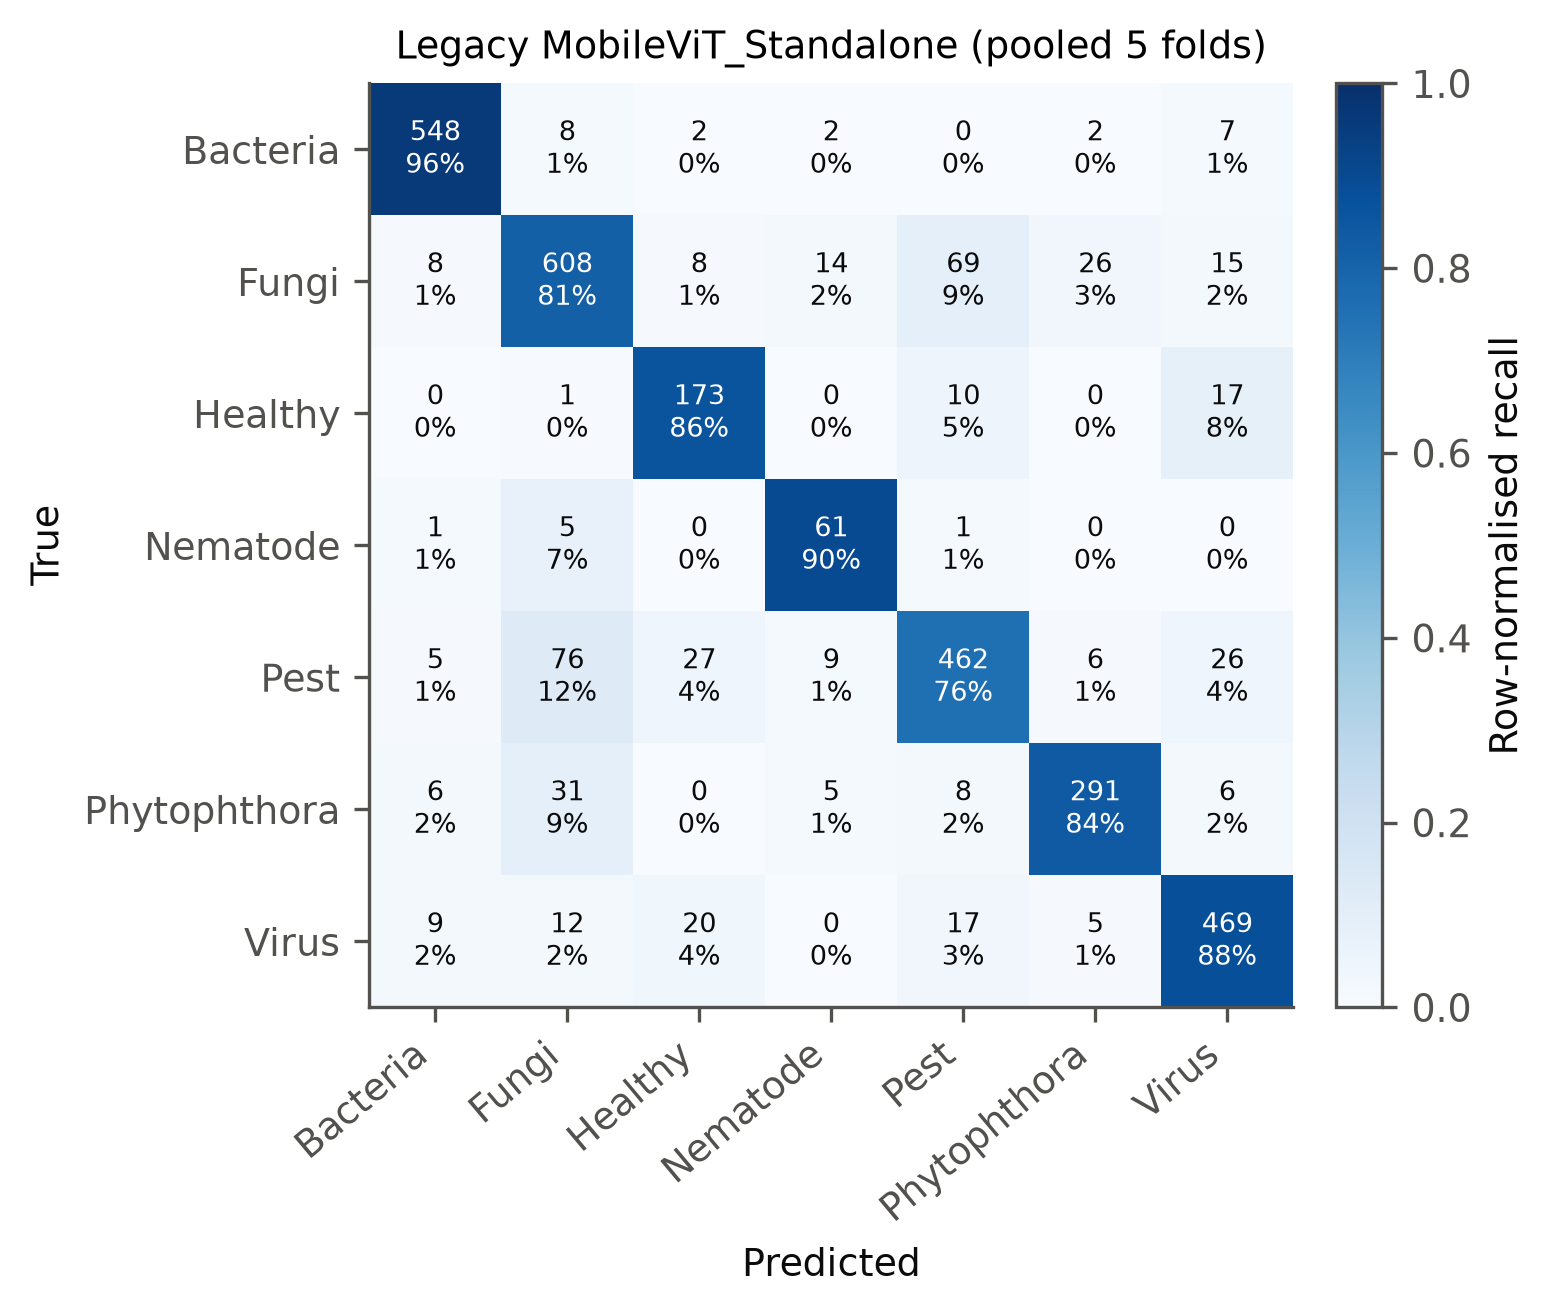
\includegraphics[width=0.75\textwidth]{figures/legacy_cm_MobileViT_Standalone.png}
  \caption{Pooled 5-fold confusion matrix of the selected legacy model
  (MobileViT-S, group-aware split). Colour encodes row-normalised recall; cells
  show counts and percentages.}
  \label{fig:legacy_cm}
\end{figure}

\subsection{Why aggressive CutMix degraded Macro-F1}
\label{sec:audit_cutmix}

\input{tables/legacy_policy}

In the policy screen (Table~\ref{tab:legacy_policy}) CutMix produced the lowest
Macro-F1 of all policies, 57.89\,\%, against 70.89\,\% without augmentation at the
same class weighting. It also nearly eliminated minority-class detection
(Nematode recall 3.1\,\%, Pest recall 30.0\,\%). We attribute this to the
mismatch between CutMix's assumptions and the structure of leaf-disease images:

\begin{enumerate}
  \item \textbf{Label/evidence misalignment.} CutMix mixes labels in proportion
  to the pasted \emph{area}, but the discriminative evidence is a few small
  lesions that cover a small fraction of the leaf. A random box removes the lesion
  in many samples, or pastes a lesion-free patch, while the target still assigns
  30--70\,\% probability to the original disease. For seven classes that share the
  same green leaf background, this injects heavy label noise.
  \item \textbf{Destroyed lesion boundaries.} Lesion margins, halos and
  concentric rings are what separate Pest from Fungi and Phytophthora. The sharp
  rectangular seams introduced by CutMix create artificial edges at exactly the
  spatial frequencies the network should learn from.
  \item \textbf{Minority starvation.} With only 52--57 Nematode images per
  training fold, the few minority samples are often pasted over or used as
  fillers, so their clean, full-label gradient signal becomes even rarer.
  \item \textbf{Slower convergence.} The screen ran for only four epochs; CutMix
  is known to need longer schedules. Part of the gap is therefore an
  under-training effect, but the direction is consistent with points 1--3. MixUp
  lost a smaller 1.6\,pp, which is consistent with the view that
  globally blending two whole leaves keeps lesion morphology intact while CutMix
  does not.
\end{enumerate}

These observations motivate the augmentation policy of ASMOE~V2: geometric
transforms that preserve lesions (rotation $\pm 20^\circ$, mild affine, flips),
mild photometric jitter (brightness and contrast $0.15$), and \emph{mild} MixUp
($\alpha = 0.2$, $\lambda \ge 0.5$, applied to half of the batches), with
CutMix removed entirely.

\subsection{Training-budget bottleneck}
\label{sec:audit_budget}

The learning curves of the final legacy CV (Fig.~\ref{fig:legacy_curves}) show
that the selected model was still improving when training stopped: the best
epochs were 12, 14, 13, 13 and 9 under a 14-epoch cap, and the training loss
($\approx 0.37$--$0.40$) was still close to the validation loss
($\approx 0.41$--$0.50$). The screening stages used only four epochs, so the
policy and architecture decisions were taken on under-trained models. ASMOE~V2
therefore uses a two-stage schedule with up to 45 epochs and patience-based early
stopping on Macro-F1.

\begin{figure}[h]
  \centering
  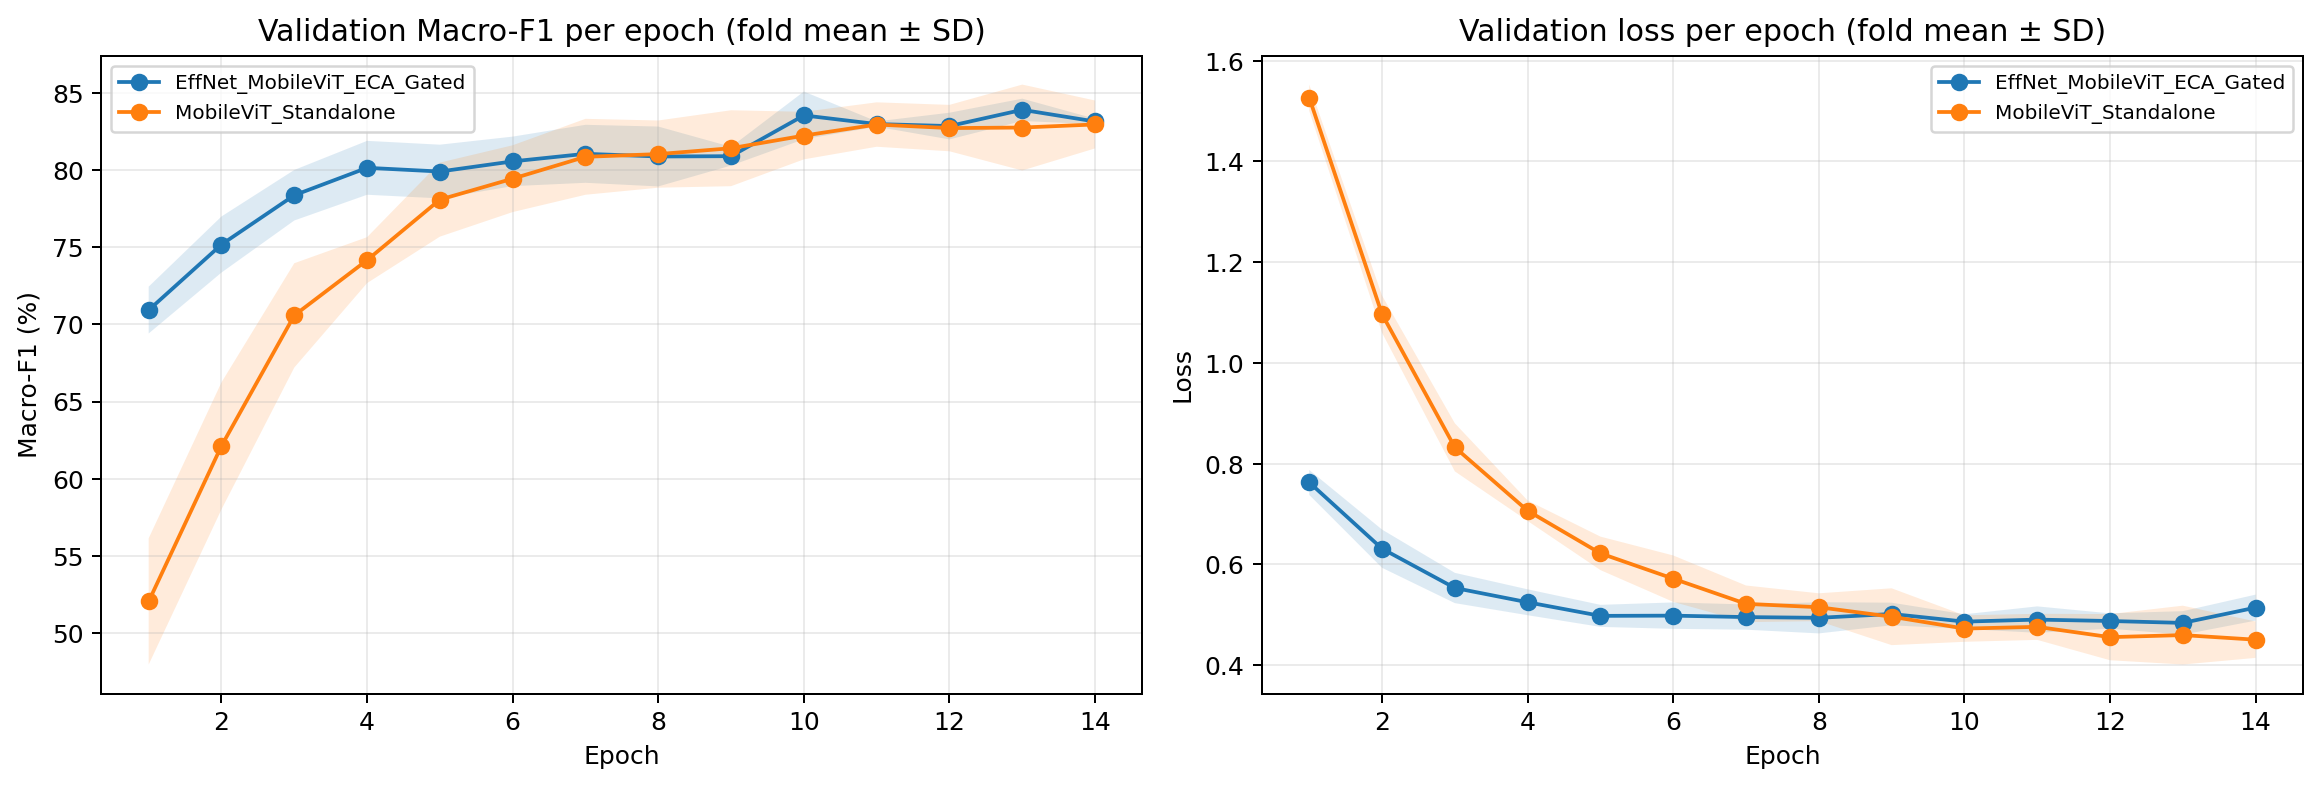
\includegraphics[width=\textwidth]{figures/legacy_learning_curves.png}
  \caption{Legacy final-CV learning curves (fold mean $\pm$ SD). Both models
  were still improving when the epoch cap was reached.}
  \label{fig:legacy_curves}
\end{figure}

\subsection{Summary of bottlenecks}
\begin{enumerate}
  \item Class imbalance of $11\times$ with re-weighting-induced false positives for Nematode and Healthy.
  \item Label noise: 6 cross-class byte duplicates (all involving Pest), 49 redundant copies, 27 near-duplicate bursts; leakage under random splits.
  \item Fine-grained Pest/Fungi/Phytophthora confusion that $224$\,px inputs cannot resolve.
  \item Augmentation that destroys lesion evidence (CutMix).
  \item Under-training (best epoch at or near the 14-epoch cap) and screening decisions taken after only four epochs.
  \item Homogeneous, lightweight backbones (4.9--10.5\,M parameters) with no global-context expert.
\end{enumerate}
